\section{UDP protocol}

\subsection{UDP packet의 의미}
    UDP User Datagram Protocol이라는 이름에서도 알 수 있듯이 데이터그램 방식을 사용하는 프로토콜이기 때문에 애초에 각각의 패킷 간의 순서가 존재하지 않는 독립적인 패킷을 사용한다. 

    또한 데이터그램 방식은 패킷의 목적지만 정해져있다면 중간 경로는 어딜 타든 신경쓰지 않기 때문에 종단 간의 연결 설정 또한 하지 않는다. 
    
    이에따라 단순히 datagram을 일방적으로 보내기 때문에 protocol의 기능을 담은 header의 field가 tcp와 비교해보았을때 단순하다.\\
    \vspace{-4mm}  
    \begin{figure}[!h]\centering
		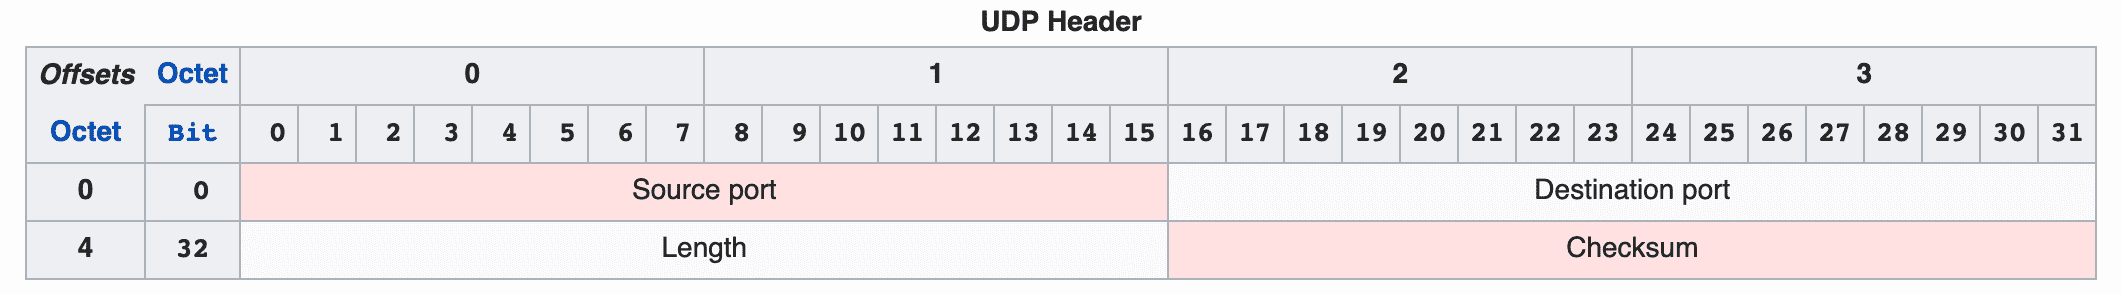
\includegraphics[width=.9\textwidth]{image/week01/2-1-1.png}
		\caption{\small UDP Header Diagram}
		\vspace{-10pt}
    \end{figure}
    
    \vspace{-2mm}
    \subsubsection*{Source Port / Destination Port}
    Invitor 와 reciver 각각의 port 정보.
    \subsubsection*{Total Length}
    헤더와 데이터를 합한 사용자 데이터그램의 전체 길이의 정보. Packet 이 아닌 Datagram을 전송하는 UDP의 경우 데이터그램의 헤더인 8바이트부터 65507바이트 사이의 값을 가진다.
    \subsubsection*{Checksum}
    TCP의 checksum field와 동일하다.헤더와 데이터를 모두 포함한 사용자 데이터그램 전체에 대해 오류를 탐지한다.
    